\documentclass[a4paper,14pt]{extarticle} % the default article class is limited to 12pt, but you can go up to 14, 17 or 20 points if you use the extarticle class:
\usepackage{cmap} % make LaTeX PDF output copy-and-pasteable
\usepackage[T2A]{fontenc}
\usepackage[utf8]{inputenc}
\usepackage[english,ukrainian]{babel}

\usepackage{amssymb,amsfonts,mathtools,amsmath,cite,enumerate,float}
\usepackage{indentfirst} % set an additional space before a paragraph at the begining of new section
\usepackage{setspace}
\usepackage{textcomp}

\usepackage{geometry} 
\geometry{left=1.25cm}
\geometry{right=1.25cm}
\geometry{top=1cm}
\geometry{bottom=2cm}

\usepackage[table,xcdraw,dvipsnames]{xcolor}
\usepackage{color}
% 1) tutorial about xcolor:  https://www.overleaf.com/learn/latex/Using_colours_in_LaTeX
% 2) huge tutorial about xcolor: https://latex-tutorial.com/color-latex/ 
% 3) RGB calculator: https://www.w3schools.com/colors/colors_rgb.asp

\usepackage{hyperref}
\definecolor{linkcolor}{HTML}{0000FF}
\definecolor{urlcolor}{HTML}{0000FF} 
\hypersetup{pdfstartview=FitH, linkcolor=linkcolor, urlcolor=urlcolor, colorlinks=true}

\usepackage{graphicx}
\usepackage{wrapfig}
\graphicspath{{Screenshots/}} % path to images

\parskip=1mm %space between paragraphs

\usepackage{listings} % for code

\lstset{
    frame=single, %lines
    language=Python,
    aboveskip=3mm,
    belowskip=3mm,
    columns=flexible,
    basicstyle={\small\ttfamily},
    numbers=left,
    numberstyle=\tiny\color{gray},
    commentstyle=\color{OliveGreen},
    stringstyle=\color{Mahogany},
    morestring=[b]''',
    showstringspaces=false,
    keywordstyle=\bfseries\color{blue},
    emph={[1]import, as, for, return}, emphstyle={[1]\bfseries\color{magenta}},
    emph={[2]range, plotting}, emphstyle={[2]\bfseries\color{brown}},
    breaklines=true,
    breakatwhitespace=true,
    tabsize=4
}

\begin{document}

\begin{titlepage}
    \newpage

    \begin{minipage}[c]{\linewidth}

        \newlength{\maxpreambula}
        \settowidth{\maxpreambula}{\small{<<Київський політехнічний інститут імені Ігоря Сікорського>>}}    

        \hspace{5cm}\parbox{\maxpreambula}{
            \begin{spacing}{1.1}\small{
                Міністерство освіти і науки України \\
                Національний технічний університет України \\
                <<Київський політехнічний інститут імені Ігоря Сікорського>> \\
                Навчально-науковий фізико-технічний інститут }
            \end{spacing}
        }
            
        \vspace*{-2.35cm}
        \hspace*{1.5cm}
        
\includegraphics[width=0.13\paperwidth]{kpi_emblem.png}

    \end{minipage}
    
    \vspace{\fill}
    
    \begin{center}
        \begin{spacing}{1.5}
            \textbf{\Large{Реалізація EM-алгоритму}} \\ 
            \vspace{1cm}\textbf{\normalsize{предмет <<Марковські моделі та їхнє застосування>>}}
        \end{spacing}
    \end{center}
    
    \vspace{\fill}
    
    \newlength{\maxname}
    \settowidth{\maxname}{\small{Цибульник Антон Владиславович}}

    \hfill\parbox{\maxname}{
        \begin{spacing}{1.1}
            \small{\textbf{Роботу виконав:}} \\ 
            \small{Студент групи ФІ-91,} \\
            \small{Цибульник Антон Владиславович} \\
        \end{spacing}
    }

    \hfill\parbox{\maxname}{
        \begin{spacing}{1.1}
            \small{\textbf{Роботу перевірила:}} \\ 
            \small{Ніщенко Ірина Іванівна} \\
        \end{spacing}
    }

    \vspace{0.5cm}

    \begin{center}
        \small{2022}
    \end{center}
    
\end{titlepage}

%\tableofcontents

\newpage

%\addcontentsline{toc}{section}{Мета}
\section*{Мета}

Ознайомитись з використанням AWS Simple Storage Service (S3).

%\addcontentsline{toc}{section}{Завдання}
\section*{Завдання} 

\begin{itemize}
    \item Створити бакет S3;
    \item Налаштувати доступ до нього з інстансу, створеного у попередній лабораторній роботі;
    \item Ознайомитись зі способами взаємодії з ним.
\end{itemize}

\section*{Хід виконання роботи}

\subsection*{0. Підготовчий етап}

\subsubsection*{Створення бакету}

Створення бакету S3 можливе різними способами. У цій роботі я користувався AWS Command Line Interface (AWS CLI).
Спершу слід встановити власне засоби AWS CLI на інстанс, доступ до якого можна отримати, зробивши аналогічні 
кроки, як це зазначалося у 3 пункті Лабораторної роботи \textnumero1. Тепер встановимо AWS CLI, ввівши команду
\[ \text{\texttt{sudo apt install awscli}} \]

Наступним кроком вкажемо усі необхідні для подальшої роботи параметри через команду \texttt{aws configure}. Для 
цього спочатку створимо окремого користувача на інстансі. Зробити це можна за допомогою розділу Identity and 
Access Management (IAM). Знайшовши цей розділ самостійно або перейшовши за 
\href{https://us-east-1.console.aws.amazon.com/iamv2/home?region=us-east-1#/home}{посиланням}, послідовно 
обираємо вкладки <<IAM resources>> $\rightarrow$ <<Users>> $\rightarrow$ <<Add users>>.

Крок за кроком проходимо п'ять етапів створення користувача, як це зображено на Рис.~\ref{fig:creation step1} та 
Рис. \ref{fig:creation step4}. На кінець отримуємо шукані параметри Access key ID та Secret access key новоствореного
юзера. Скориставшись \href{https://docs.aws.amazon.com/cli/latest/userguide/cli-configure-files.html}{інструкцією}, 
нарешті виконуємо команду \texttt{aws configure} через консоль (Рис. \ref{fig:aws configure}).

\begin{figure}[H]
    \center{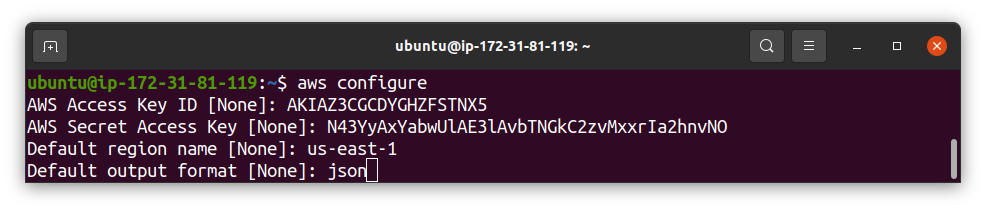
\includegraphics[width=1\linewidth]{aws 0.3.png}}
    \caption{Виконання команди aws configure}
    \label{fig:aws configure}
\end{figure}

\begin{figure}[H]
    \center{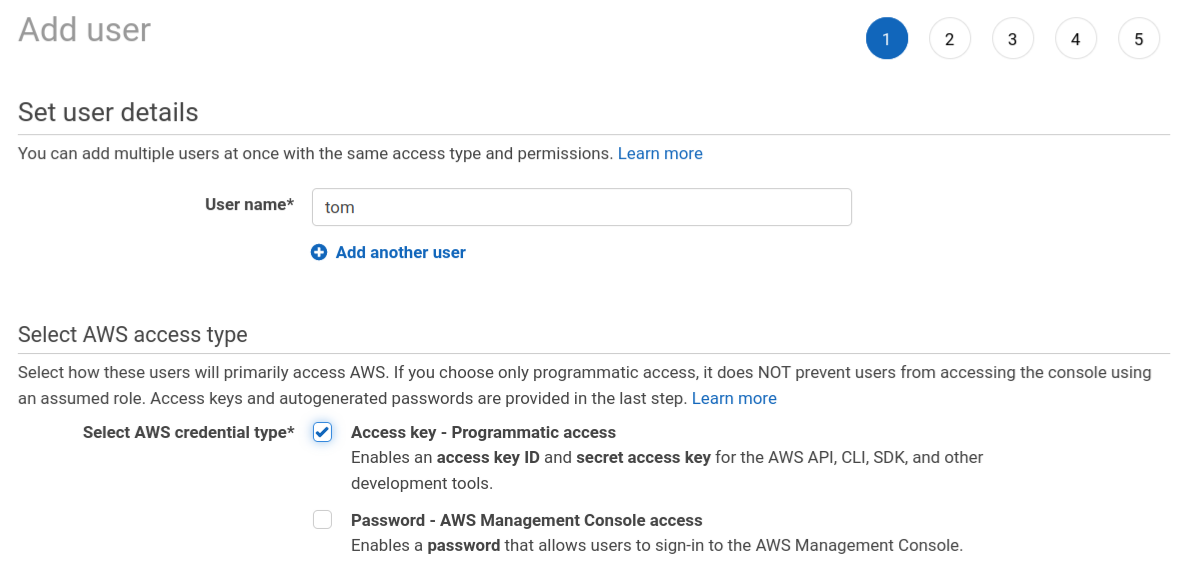
\includegraphics[width=1\linewidth]{aws 0.1.png}}
    \caption{Перший етап створення користувача}
    \label{fig:creation step1}
\end{figure}

\begin{figure}[H]
    \center{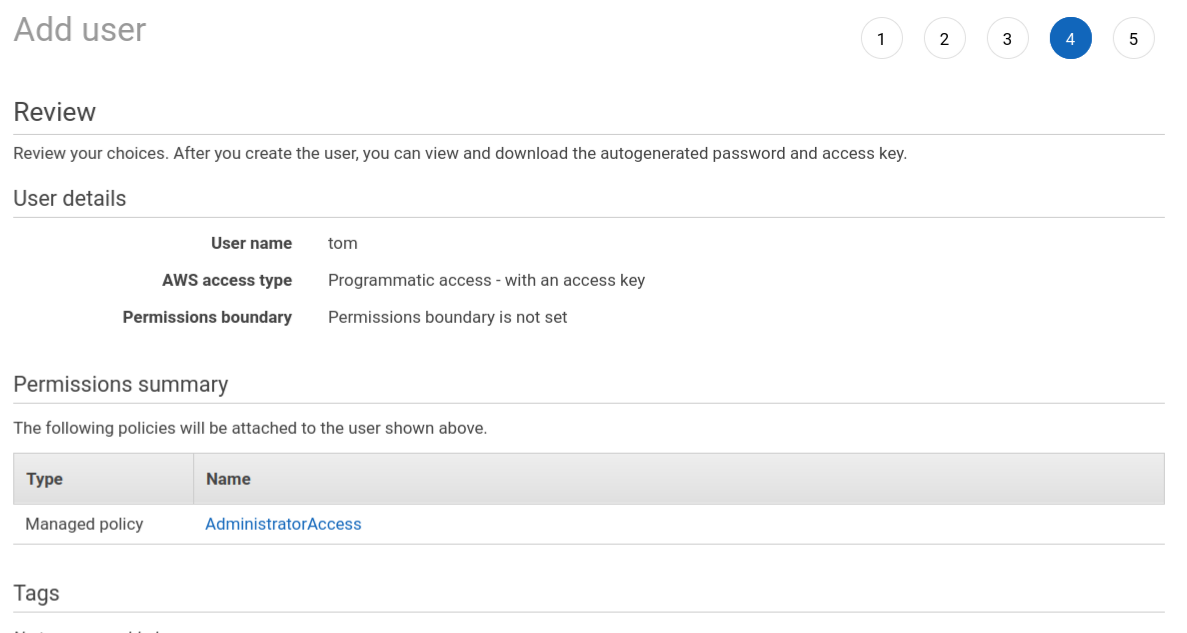
\includegraphics[width=1\linewidth]{aws 0.2.png}}
    \caption{Передостанній етап створення користувача}
    \label{fig:creation step4}
\end{figure}

Фінальним кроком цього підрозділу створюємо новий бакет (Рис. \ref{fig:creation of bucket}) консольною 
командою
\[ \texttt{aws s3 mb s3://bucket01my} \]

Слід зауважити, що ім'я бакету має бути унікальним. Знайшовши розділ <<S3>> 
самостійно або перейшовши за 
\href{https://s3.console.aws.amazon.com/s3/buckets?region=us-east-1}{посиланням}, переконуємося, що бакет 
створений і є у переліку (Рис. \ref{fig:list of buckets}). 

\begin{figure}[H]
    \center{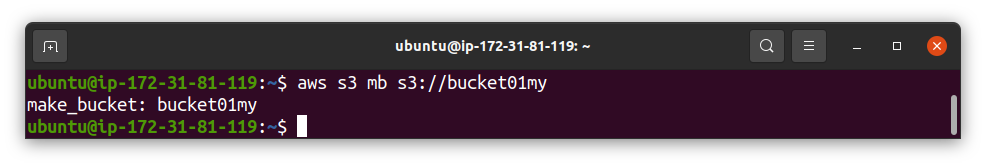
\includegraphics[width=1\linewidth]{aws 0.4.png}}
    \caption{Створення бакету}
    \label{fig:creation of bucket}
\end{figure}

\begin{figure}[H]
    \center{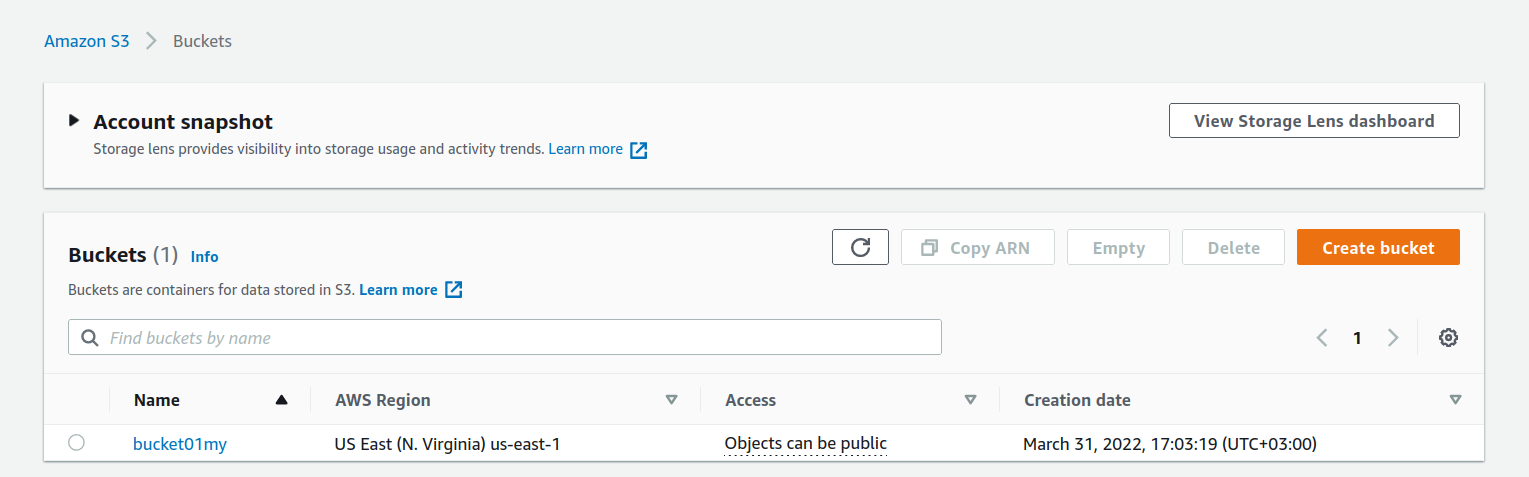
\includegraphics[width=1\linewidth]{aws 0.5.png}}
    \caption{Перелік бакетів}
    \label{fig:list of buckets}
\end{figure}

\subsubsection*{Початок роботи з jupyter notebook}

Для налаштування Python API потрібно встановити пакетний менеджер pip. Піс\-ля оновлення дерева пакетів 
виконуємо команди
\begin{align*}
    &\texttt{sudo apt update} \\
    &\text{\texttt{sudo apt install python3-pip}}
\end{align*}

Процес завантаження зображено на Рис. \ref{fig:downloading pip}. Надалі завантажуємо на інстанст власне jupyter notebook:
\[ \text{\texttt{sudo pip3 install jupyter notebook}} \]

Якщо виникли проблеми із цілісним завантаженням jupyter notebook, варто спробувати запустити іншу команду встановлення:
\[ \text{\texttt{sudo pip3 install {-}{-}upgrade {-}{-}force-reinstall {-}{-}no-cache-dir jupyter}} \]

Постає завдання: запустити щойно встановлений jupyter notebook на інстансі та працювати з ним з локального 
робочого місця. Виконуємо команди (як на Рис. \ref{fig:localhost}):
\begin{align*}
    &\texttt{jupyter notebook {-}{-}no-browser {-}{-}port 8889} && \text{на інстансі} \\
    &\text{\texttt{ssh -i lab.pem -N -f -L localhost:8888:localhost:8889}} && \text{локально}
\end{align*}

\begin{figure}[H]
    \begin{minipage}[H]{1\linewidth}
        \center{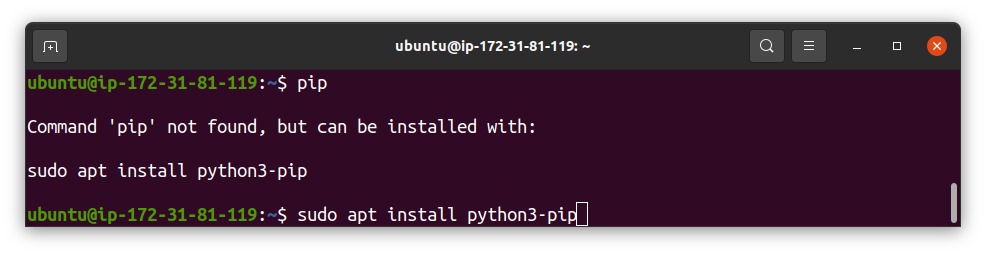
\includegraphics[width=1\linewidth]{pip 0.6.png}}
    \end{minipage}
    \vfill
    \begin{minipage}[H]{1\linewidth}
        \center{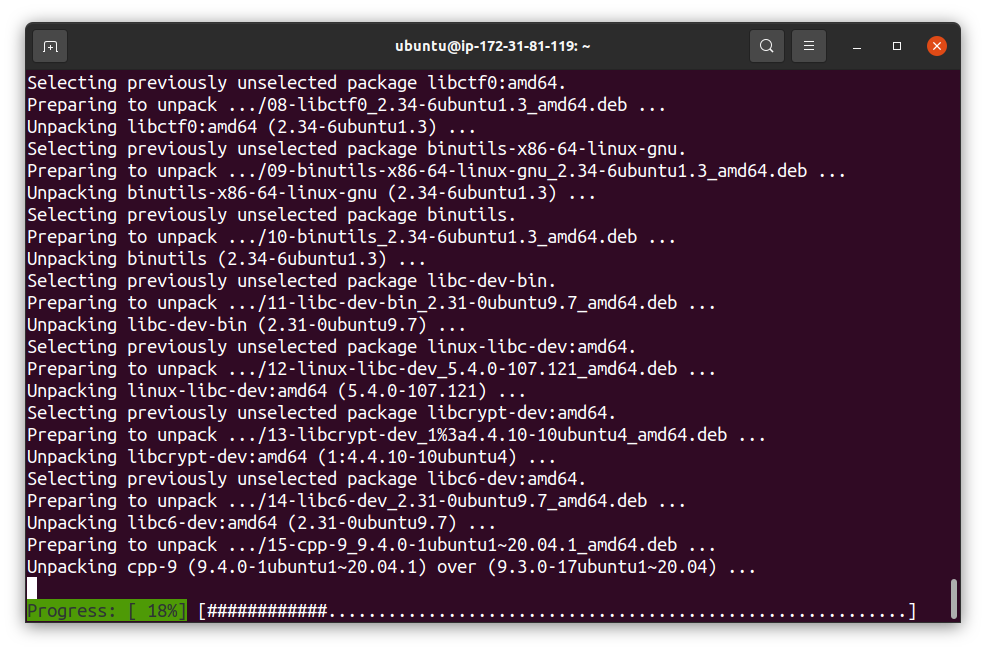
\includegraphics[width=1\linewidth]{pip 0.7.png}}
        \caption{Встановлення pip}
        \label{fig:downloading pip}
    \end{minipage}
\end{figure}

Завантаживши pip (Рис. \ref{fig:downloading pip}) й встановивши віддалений доступ до jupyter notebook 
(Рис. \ref{fig:localhost}), переходимо за посиланням \url{http://localhost:8888/} й вказуємо token. Відтак відкриваємо 
дерево папок й створюємо новий файл \texttt{Lab2.ipynb} (Рис. \ref{fig:jupyter notebook}).

\begin{figure}[H]
    \center{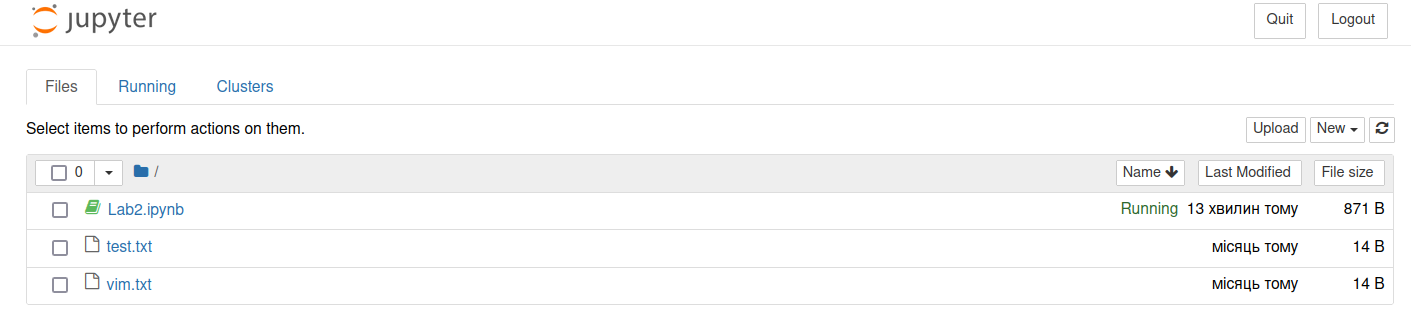
\includegraphics[width=1\linewidth]{pip 0.10.png}}
    \caption{Сховище jupyter notebook}
    \label{fig:jupyter notebook}
\end{figure}

\begin{figure}[H]
    \begin{minipage}[H]{1\linewidth}
        \center{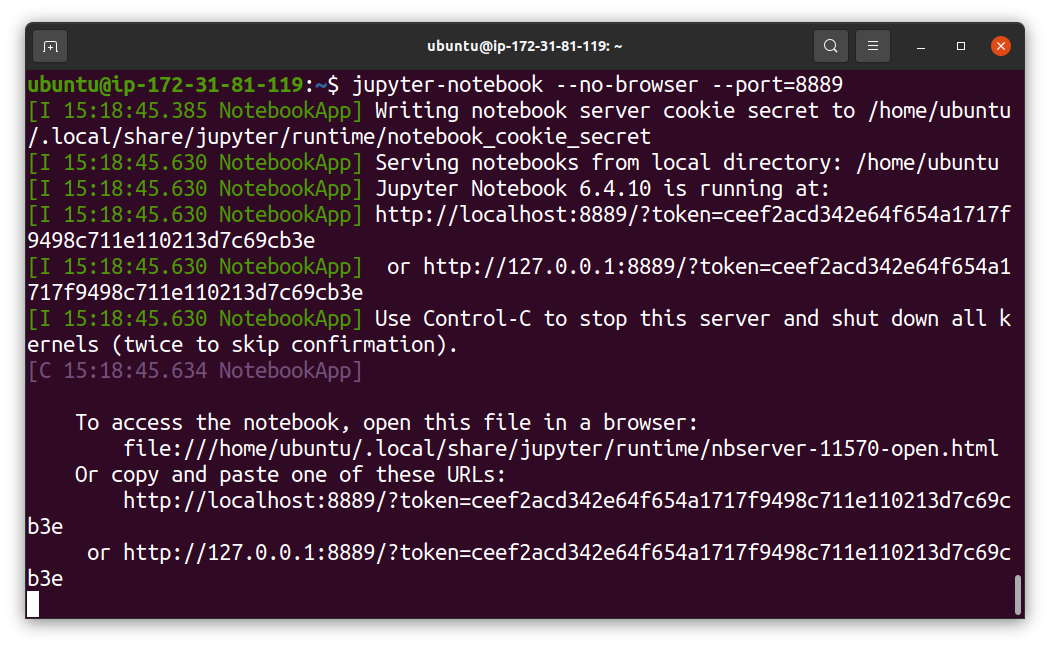
\includegraphics[width=1\linewidth]{pip 0.8.png}}
    \end{minipage}
    \vfill
    \begin{minipage}[H]{1\linewidth}
        \center{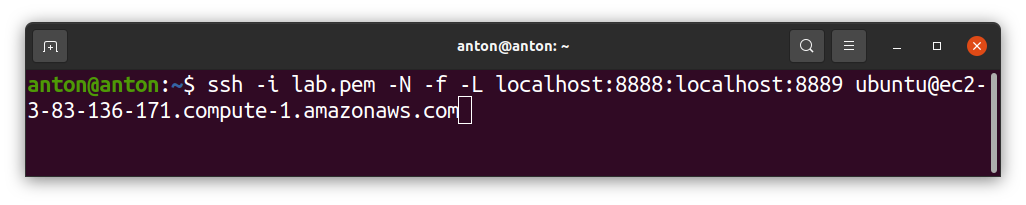
\includegraphics[width=1\linewidth]{pip 0.9.png}}
        \caption{Віддалений доступ до jupyter notebook}
        \label{fig:localhost}
    \end{minipage}
\end{figure}

\subsection*{1. Отримання даних щодо курсу гривні}

Завданням етапу є програматичне отримання даних у JSON-форматі на інстанс, а саме: інформації щодо курсу гривні 
за 2021 рік. Перейшовши за \href{https://bank.gov.ua/ua/open-data/api-dev}{посиланням}, опиняємося на сторінці 
Національного банку України. Послідовно обираємо 
\begin{align*}
    &\rightarrow \text{<<API для розробників>>} \\ 
    &\rightarrow \text{<<1. Офіційний курс гривні до іноземних валют ... >>} \\ 
    &\rightarrow \text{<<Інструкція до сервісу отримання курсів гривні до іноземних валют ... >>}
\end{align*}

Клікаємо на посилання, яке має вид
\url{https://bank.gov.ua/NBUStatService/v1/statdirectory/exchangenew?json}, маючи змогу переглянути таким 
чином дані про курс гривні. Додаючи до посилання фрагмент \texttt{\&date=20210110} можна отримати інформацію про курс на 
конкретну дату (наприклад, на 10.01.2021). Наступним кроком буде програматичний етап: зчитування знайдених даних засобами 
Python через хмарний jupyter notebook.

Підключимо такі дві бібліотеки: \texttt{requests} для роботи із запитами та \texttt{json} для перетворення й 
збереження відповідного формату файлів. За допомогою методу request.get() отримаємо дані з сайту, постіпово крок за 
кроком зчитуючи й записуючи інформацію про 10 число кожного місяця (Лістинг \ref{get data}, рядки 4-16).
 
\lstinputlisting[firstline=1, lastline=16, label = get data, caption = Отримання даних]{Code/s3.py}

Наступним кроком перетворимо отриману інформацію з \texttt{json} рядка у \texttt{json} файл. Тобто, фактично, 
завантажимо всі дані на інстанст у вигляді файлу, який назвемо \texttt{request.json} (Лістинг \ref{download json}, рядки 18-21). 


Для перевірки візулізуємо таблицю даних за допомогою бібліотеки \texttt{pandas}, завантаження якої зображено на 
Рис. \ref{fig:download pandas}. Отримали таблицю із спільною інформацією про усі курси валют для кожного із 
дванадцяти місяців. Результати самої візуалізації можна побачити на Рис. \ref{fig:show me your data}, а саме: 
перші й останні шість рядків.

\lstinputlisting[firstnumber = 18, firstline=18, lastline=27, label = download json, caption = Завантаження даних]{Code/s3.py}

\begin{figure}[H]
    \center{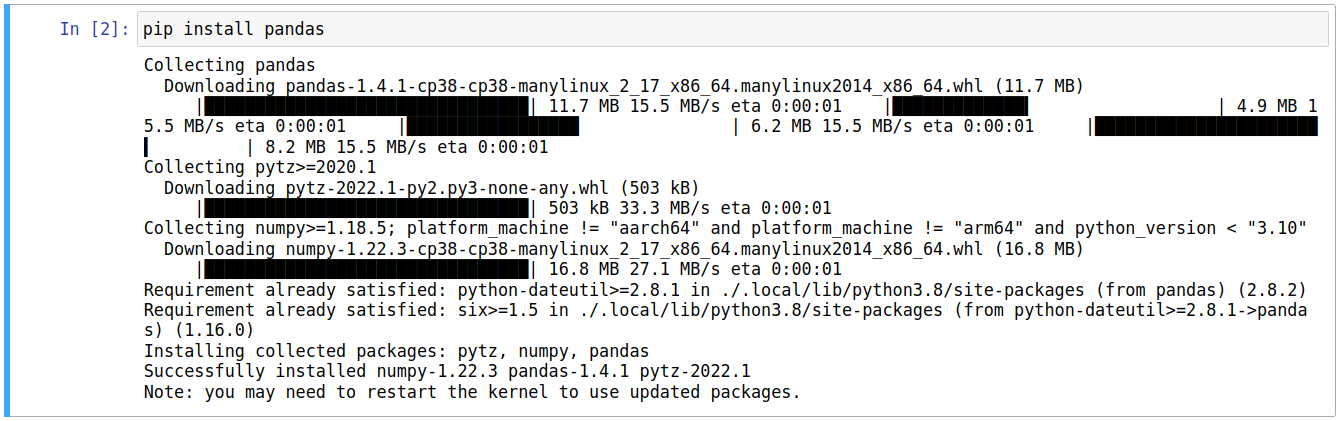
\includegraphics[width=1\linewidth]{1.1.png}}
    \caption{Завантаження бібліотеки pandas}
    \label{fig:download pandas}
\end{figure}

\begin{figure}[H]
    \begin{minipage}[H]{0.49\linewidth}
        \center{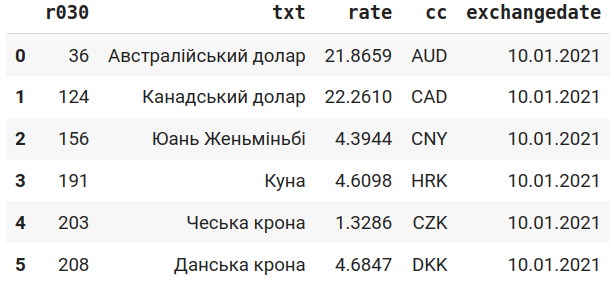
\includegraphics[width=1\linewidth]{1.2.1.png}}
    \end{minipage}
    \hfill
    \begin{minipage}[H]{0.49\linewidth}
        \center{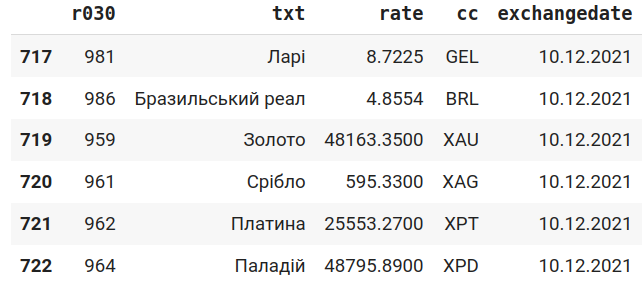
\includegraphics[width=1\linewidth]{1.2.2.png}}
    \end{minipage}
    \caption{Перші й останні рядки таблиці даних}
    \label{fig:show me your data}
\end{figure}

\subsection*{2. Конвертація json-файлу у csv-файл}

Для поставленого завдання виконаємо ряд команд (Лістинг \ref{conver to csv}), які дозволять власне конвертувати 
файл й зберегти його на інстансі. Перевірку збереження можна провести, відкривши сховище jupyter notebook 
(Рис \ref{fig:jupyter notebook}).

\lstinputlisting[firstnumber = 29, firstline=29, lastline=30, label = conver to csv, caption = Конвертація файлу]{Code/s3.py}

\subsection*{3. Вивантаження інформації на S3}
\label{section 5}

Вивантажимо отриманий файл \texttt{request.csv} з інстансу на бакет. Зробимо це за допомогою 
\href{https://awscli.amazonaws.com/v2/documentation/api/latest/reference/s3/cp.html}{команди} \texttt{cp}, 
яка є одним з 
\href{https://awscli.amazonaws.com/v2/documentation/api/latest/reference/s3/index.html}{інструментів AWS CLI}.
Насамперед завершимо сеанс підключення до хмарного ноутбуку, натиснувши в командному рядку, через який 
відбувається доступ до інстансу, комбінацію клавіш \texttt{Ctrl+C} й ввівши \texttt{yes} у діалоговому 
рядку. Тож після підготовчих кроків виконуємо команду 
\[ \texttt{aws s3 cp request.csv s3://bucket01my} \]

Перевіримо успішне виконання команди, обравши назву свого бакету (як на Рис.~\ref{fig:list of buckets}) серед 
списку усіх бакетів. Результат перевірки зображено на Рис. \ref{fig:svg on S3}.

\begin{figure}[H]
    \center{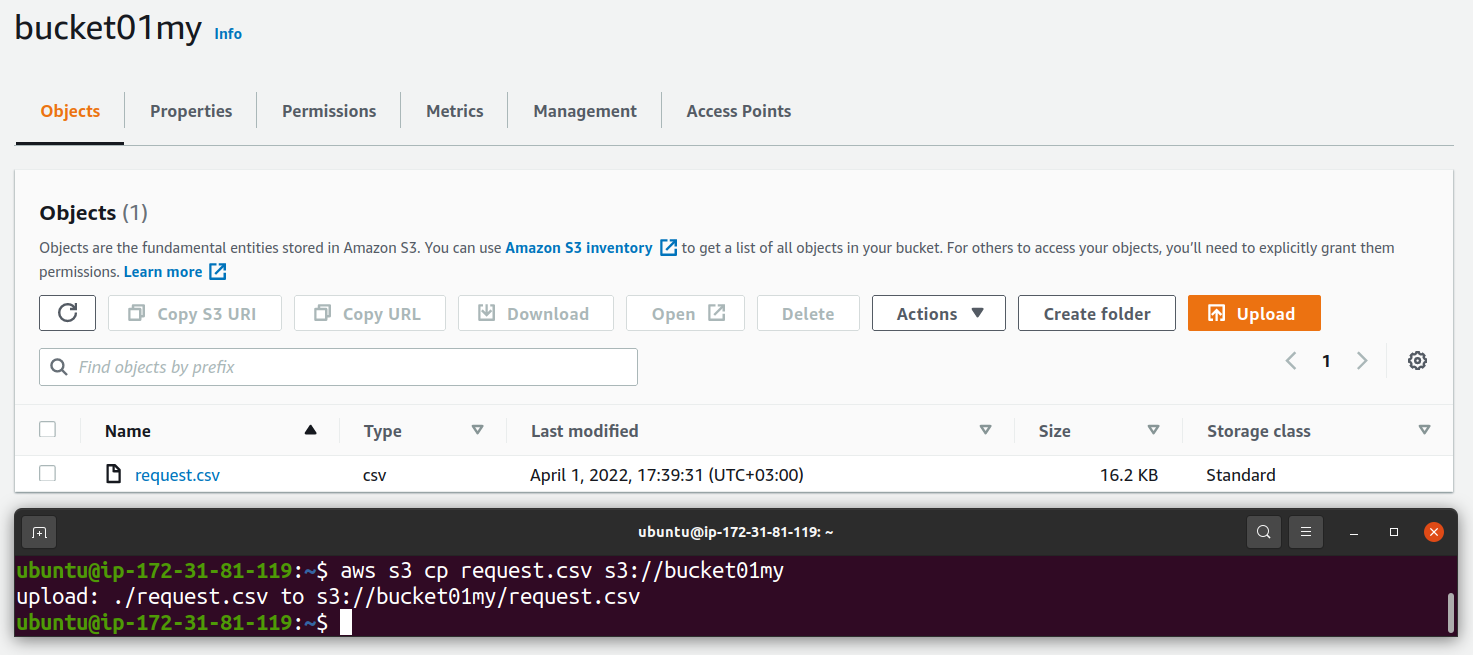
\includegraphics[width=1\linewidth]{3.png}}
    \caption{Вивантаження інформації на S3}
    \label{fig:svg on S3}
\end{figure}

\subsection*{4. Cкрипт для читання файлів з бакету}

Наразі на бакеті маємо завантажений файл \texttt{request.csv}, який зберігає дані про курс гривні за дванадцять 
місяців. Маємо намір зчитувати безпосередньо з бакету дані й працювати з ними на jupyter notebook. 

В нагоді стануть засоби мови Python. Тому перш за все знову підключаємося до хмарного ноутбуку (як це було 
зазначено на Рис.~\ref{fig:localhost}). Нас\-тупним кроком завантажуємо бібліотеку \texttt{boto3} (аналогічним 
чином, як було завантажено бібліотеку \texttt{pandas} на Рис. \ref{fig:download pandas}). Програмний етап можна 
побачити на Лістингу \ref{boto3}. 

Останнім кроком первіримо успішне виконання поставленого завдання, візуалізувавши зчитану з файлу таблицю даних 
(Лістинг \ref{boto3}, рядок 39). Результат має бути аналогічним до таблиці на Рис. \ref{fig:show me your data}. 

\lstinputlisting[firstnumber = 32, firstline=32, lastline=39, label = boto3, caption = Зчитування даних з бакету]{Code/s3.py}

\subsection*{5. Графіки курсу гривні}

Для малювання графіків застосуємо створену якраз для подібних цілей бібліотеку \texttt{matplotlib}. Попередньо 
завантаживши її, напишемо скрипт (Лістинг \ref{matplotlib}).

\lstinputlisting[firstnumber = 41, firstline=41, lastline=72, label = matplotlib, caption = Графіки курсу гривні]{Code/s3.py}

Наведемо ключове пояснення до написаної вище програми: пробігаючи циклом \texttt{for} по масиву індексів (тобто покроково по 
кожному рядку таблиці даних), висмикуємо в окремий масив інформацію про курс гривні з тих рядків, які мають 
потрібну нам валюту долара <<USD>> чи євро <<EUR>> й вказану дату (10 число кожного місяця). Надалі саме з новостворених масивів 
поточково малюємо графічні залежності. 

Технічно реалізацію виконано за допомогою таких ключових елементів:
\begin{align*}
    & \texttt{df.index} && \text{масив індексів усіх рядків} \\
    & \texttt{df.loc[i]} && \text{атрибут для пробігу по i-му рядкку} \\
    & \texttt{plt.figure()} && \text{встановлення розмірів зображення} \\
    & \texttt{plt.subplot()} && \text{поєдняння двох графіків на одному малюнку} \\
    & \texttt{plt.grid()} && \text{розмірна сітка} \\
\end{align*}

Результати етапу зафіксовано на Рис. \ref{fig:currency}.

\begin{figure}[H]
    \center{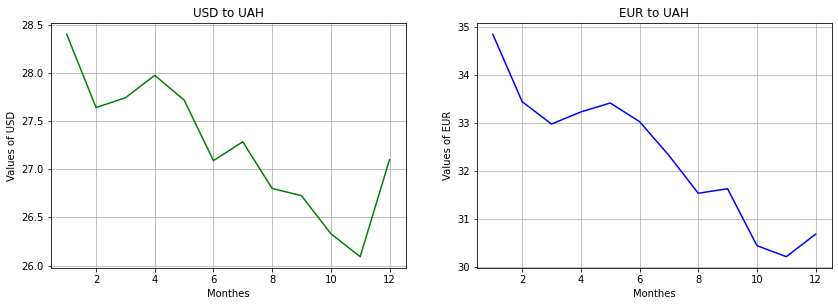
\includegraphics[width=1\linewidth]{5.2.png}}
    \caption{Результати візуалізації курсу гривні}
    \label{fig:currency}
\end{figure}

\subsection*{6. Збереження графіків на бакет}

Перш за все завантажимо отриманий у попередньому пункті графік на інстанс. Зробимо це за допомогою команди, 
наведеної на Лістингу \ref{matplotlib}, рядок 71. Відкривши сховище jupyter notebook, маємо переконатися в 
успішності виконання. 

Наступним етапом повторимо усі кроки пункту 3 (сторінка \pageref{section 5}), щоб отриманий графік вивантажити 
з інстансу на бакет. Щойно зазначені кроки послідовно зображено на малюнку нижче (Рис. \ref{fig:copy .png to bucket}).
Остаточний результат виконання шостого пункту зазначено на Рис. \ref{fig:png on s3}.

\begin{figure}[H]
    \center{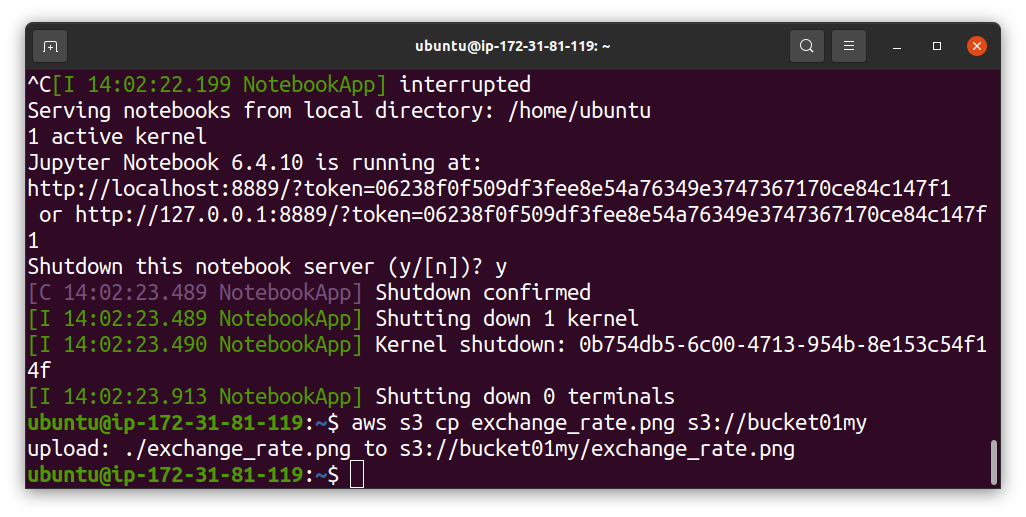
\includegraphics[width=1\linewidth]{6.1.png}}
    \caption{Вивантаження малюнка на бакет}
    \label{fig:copy .png to bucket}
\end{figure}

\begin{figure}[H]
    \center{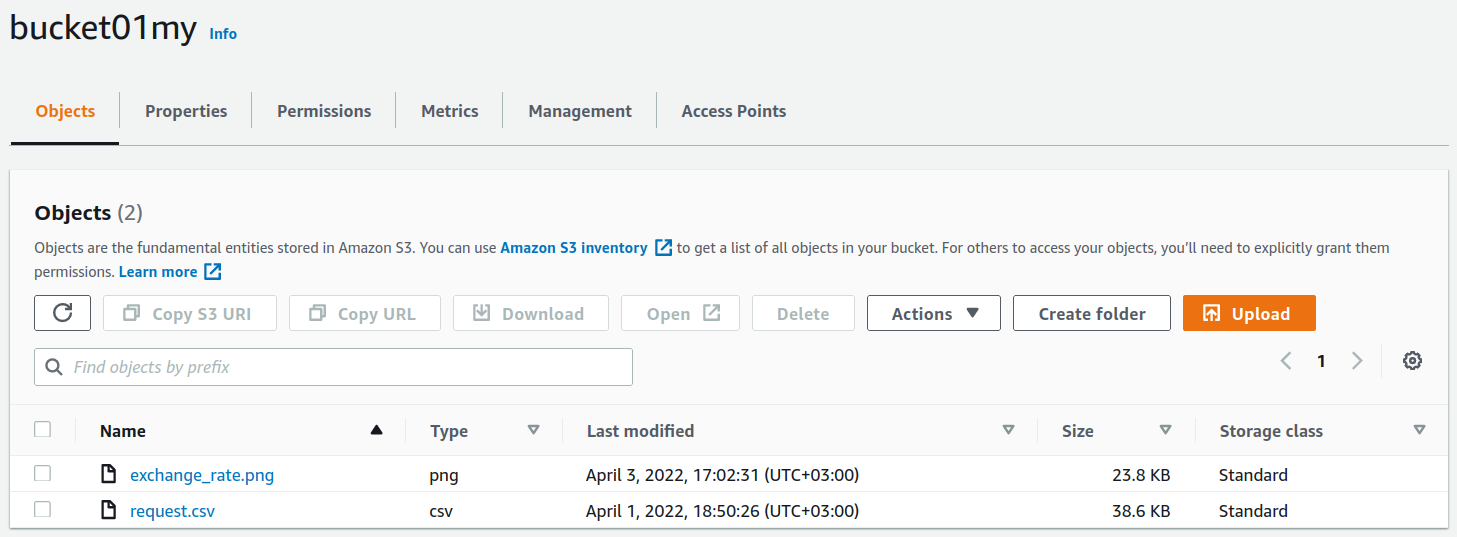
\includegraphics[width=1\linewidth]{6.2.png}}
    \caption{Результат вивантаження малюнка на бакет}
    \label{fig:png on s3}
\end{figure}

\subsection*{7. Перелік проблем протягом виконання роботи}

\begin{enumerate} [Пункт 1:]
    \item [Пункт 0:] 
        \begin{enumerate} 
            \item При створенні бакету інструментами AWS CLI лише з п'ятої-десятої спроби вдалося підібрати 
            унікальне ім'я новоствореного бакету. Крім того, наскільки я зрозумів, деякі імена були неприйнятними 
            через надто велику довжину символів;

            \item Як вже зазначалося при описі підготовчого кроку, у мене виникла проблема iз цiлiсним 
            завантаженням jupyter notebook. На жаль, після застосування звичайної команди завантаження, наведеної 
            в методичних вказівках до лабораторної роботи, не вдалося віднайти усі пакети. Як я довідався 
            з відповідей на сайті \url{https://stackoverflow.com}: 
            <<It seems to me as though the installation has messed up somehow.>> Проблему вирішило застосування команди 
            \[ \text{\small\texttt{sudo pip3 install --upgrade --force-reinstall --no-cache-dir jupyter}} \]

            \item При спробі встановити віддалений зв'язок з хмарним ноутбуком з локального сховища (тобто 
            при створенні SSH-тунелю), рекомендації в методичці для операційної системи Linux 
            вказували додати компонент виду \texttt{ubuntu@54.71.56.14} до основної команди. На жаль, результуюча 
            команда просто не виконувалася. Натомість довелося скористатися вказівками до операційної системи 
            Windows, де рекомендувалося додати рядок виду \texttt{ubuntu@Public\_IPv4\_adress}.
        \end{enumerate}

    \item [Пункт 1:] Під час початку роботи із jupyter notebook постійно стикався з проблемою неправильного кодування 
    json рядків (стосується в основному Лістингу~\ref{get data}). Компілятор видавав повідомлення: <<JSONDecodeError>>. 
    Час від часу, перезапускаючи jupyter notebook, цю проблему вдавалося оминути й усі рядки компілювалися справно.

    \item [Пункт 3:] Замість запропонованих в методичці інструментів бібліотеки \texttt{boto3}, вирішив скористатися 
    простішою на вигляд командою \texttt{cp} інструментів AWS CLI. Із цим була пов'язана одна проблема: при повторній 
    спробі вивантажити на бакет певний файл, довелося додатково оновити усі інструменти командою 
    \[ \texttt{pip install {-}{-}upgrade awscli} \]

    \item [Пункт 5:] Основна складність, яка виникла з кодом на Лістингу \ref{matplotlib}, полягала у спробах 
    віднайти спосіб доступу до рядків таблиці. Інакше прорідити дані й відсіяти непотрібні здавалося неможливим. 
    Проблему вирішив знайдений метод \texttt{df.loc[i]}. Решта труднощів з кодом полягала у необхідності додат\-кового 
    встановлення бібліотек \texttt{pandas,boto3} та \texttt{matplotlib}.
\end{enumerate}

\end{document}